\documentclass{standalone}
\usepackage{tikz}
\usetikzlibrary{fit}

\begin{document}
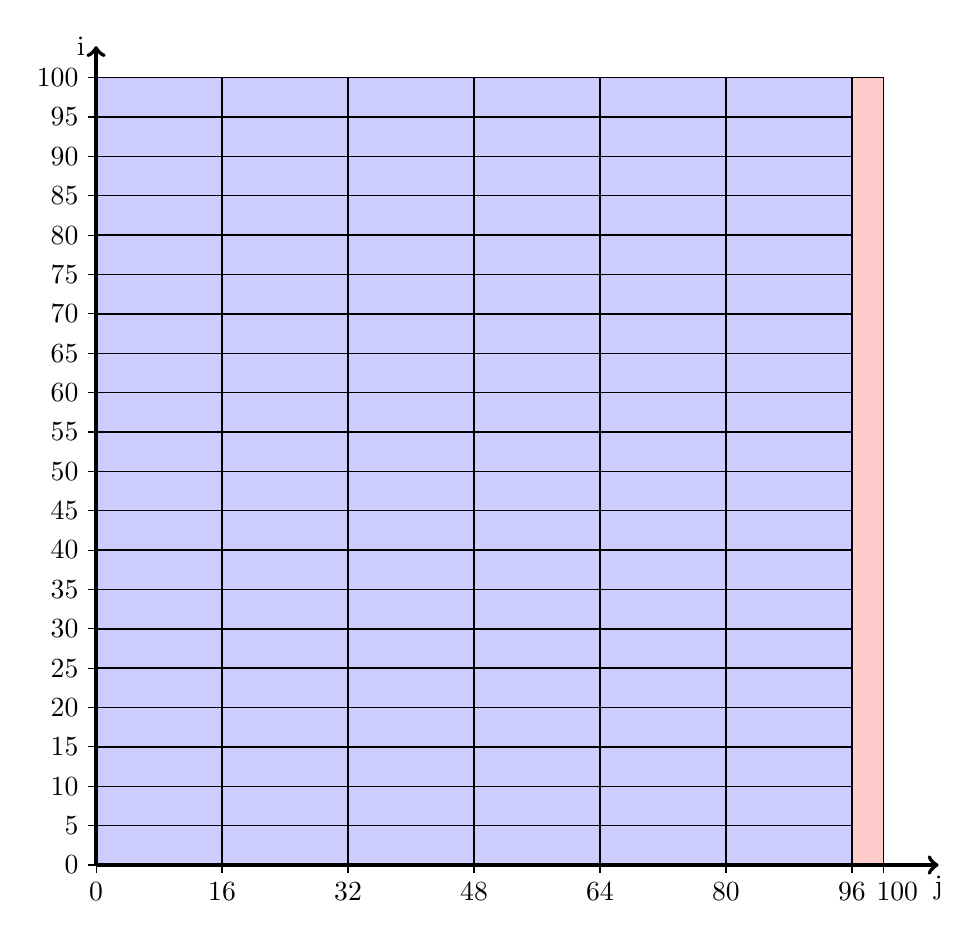
\begin{tikzpicture}
\tikzset{axis/.style={draw=black,->,line width=1.5pt}}
\tikzset{reddot/.style={fill=red,circle,inner xsep=0mm,inner ysep=0mm,minimum width=6mm,anchor=center}}
\tikzset{bluedot/.style={fill=blue,circle,inner xsep=0mm,inner ysep=0mm,minimum width=6mm,anchor=center}}
\tikzset{dot/.style={fill=black!60,circle,inner xsep=0mm,inner ysep=0mm,minimum width=0.5mm,anchor=center}}
\tikzset{completetile/.style={draw=black,->,line width=0.5pt,fill=blue!20}}
\tikzset{partialtile/.style={draw=black,->,line width=0.5pt,fill=red!20}}

\begin{scope}[x={(1mm,0mm)},y={(0mm,1mm)}]

\foreach \x in {0,16,...,80} {
    \foreach \y in {0,5,...,95} {
       \path[completetile] (\x,\y) rectangle (\x+16,\y+5);
    }
}

\path[partialtile] (96,0) rectangle (100,100);

\path[axis] (0,0) -- (100+7,0) node[below](i)  {j};
\foreach \x in {0,16,...,96} {
  \path[draw] (\x,0) -- ++(0,-0.1cm) node[below] {\x};
}
\path[draw] (100,0) -- ++(0,-0.1cm) node[below,xshift=5] {100};

\path[axis] (0,0) -- (0,100+4) node[left](j) {i};
\foreach \y in {0,5,...,100} {%
  \path[draw] (0,\y) -- ++(-0.1cm,0) node[left]() {\y};%
}

\end{scope}
\end{tikzpicture}
\end{document}
